\section{2. Euclidean Space}
% **************************

\subsection{Properties of vectors}
% ================================

Dot product, norm and distances. The dot product of two vectors \textbf{A} and
\textbf{B} can be thought as the prodcut of their magnitude times the angle between
them:

$$\mathbf{A} \cdot \mathbf{B} = \|\mathbf{A}\| \cdot \|\mathbf{B}\|cos(\theta)$$

Since $cos(\pi/2) = 0$, if the two vectors are orthogonal their dot product is
0. For example $\left[\begin{matrix}2\\0\end{matrix}\right] \cdot \left[\begin{matrix}0\\2\end{matrix}\right] = 0$

\subsubsection{Exercise 2.1.1}
% ----------------------------

Evaluate

\begin{verbatim}
import matplotlib.pyplot as plt

u= Matrix(2, 1, [-1, 3])
v= Matrix(2, 1, [2, 1])

plt.text(float(u[0])+0.2, float(u[1]), 'u', fontsize= 30, color= 'r')
plt.text(float(v[0])-0.2, float(v[1]), 'v', fontsize= 30, color= 'r')
plt.arrow(0, 0, float(u[0]), float(u[1]), lw= 3, color= 'b', head_width=0.05)
plt.arrow(0, 0, float(v[0]), float(v[1]), lw= 3, color= 'b', head_width=0.05)
plt.xlim((-1.1, 3.1))
plt.ylim((-1.1, 3.1))
plt.grid()
plt.savefig('figs/ex2_1_1.pdf')
plt.close()
\end{verbatim}

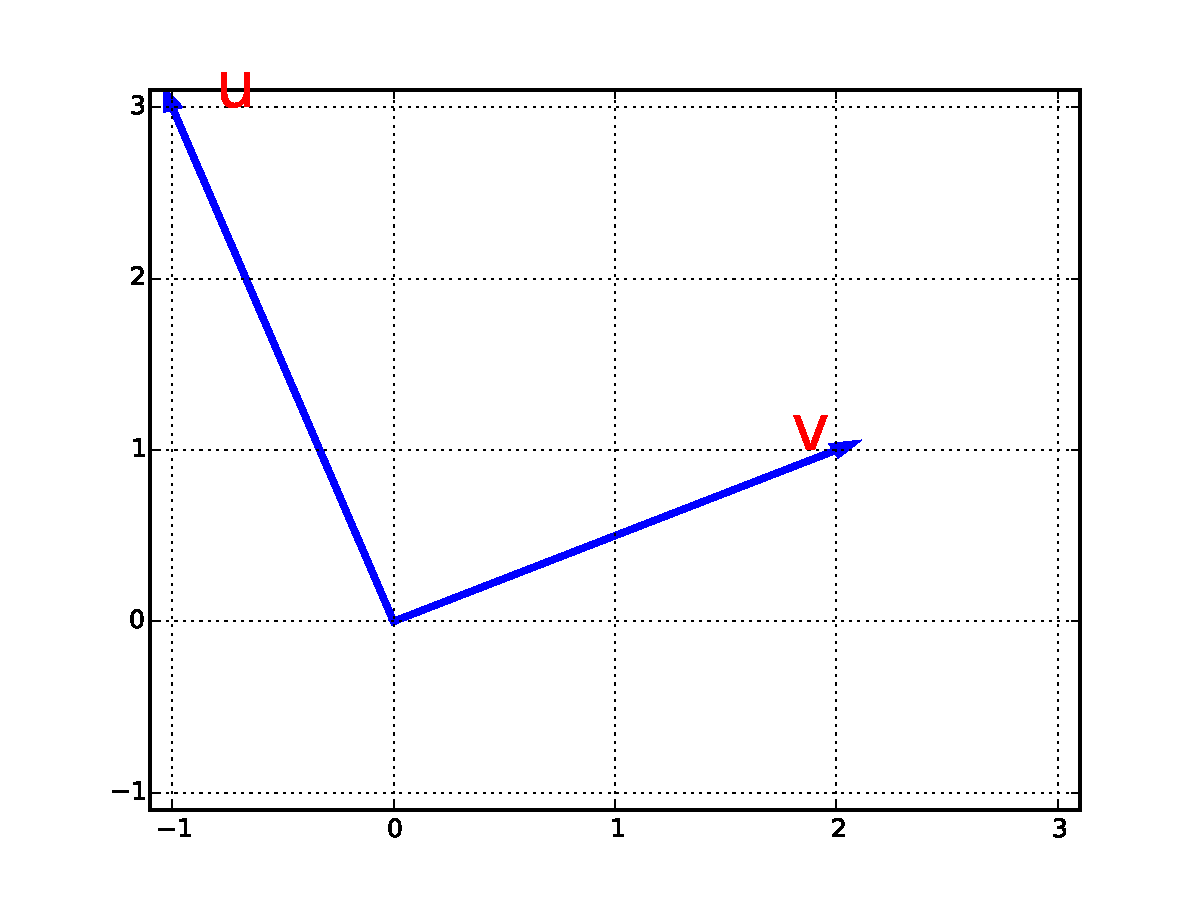
\includegraphics[width=\linewidth]{figs/ex2_1_1.pdf}

\begin{verbatim}
u.dot(v) # 1
v.dot(u) # 1
u.dot(u) # 10
v.dot(v) # 5

u.norm()            # sqrt(10)
u.norm()**2         # 10
v.norm()            # sqrt(5)
v.norm()**2         # 5
(u + v).norm()**2   # 17
(u - v).norm()      # sqrt(13)
\end{verbatim}

\subsubsection{Exercise 2.1.3}
% ----------------------------
Evaluate for
$\mathbf{u} = \left[\begin{matrix}-1\\2\\5\\-3\end{matrix}\right]$ and
$\mathbf{v} = \left[\begin{matrix}2\\-3\\-1\\5\end{matrix}\right]$

\begin{verbatim}
u= Matrix(4, 1, (-1, 2, 5, -3))
v= Matrix(4, 1, (2, -3, -1, 5))
\end{verbatim}

\textbf{Dot product}:

\begin{verbatim}
v.dot(u)    # -28
u.dot(v)    # -28  
v.dot(v)    # 39
u.dot(u)    # 39
\end{verbatim}

Note that commutative property hold. NB \textbf{\texttt{u * v}} raises \texttt{\textcolor{red}{ShapeError: Matrices size mismatch.}}

\textbf{Norm} (\emph{symbol}: $\|u\|$, $\|u + v\|$, $\|u\|^2$, etc)

\begin{verbatim}
u.norm()            # sqrt(39)
u.norm()**2         # 39
v.norm()            # sqrt(39)
v.norm()**2         # 39
(u + v).norm()**2   # 22
\end{verbatim}

\textbf{Distance} $d(u, v) = \| u - v \|$

\begin{verbatim}
(u - v).norm() # sqrt(134)
(v - u).norm() # sqrt(134)
\end{verbatim}

\subsubsection{Exercise 2.1.6}
% ----------------------------

Plot and compute for $\mathbf{u} = \left[\begin{matrix}7\\-2\end{matrix}\right]$
and $\mathbf{v} = \left[\begin{matrix}-5\\3\end{matrix}\right]$

$$\|\mathbf{u} + \mathbf{v} \| = \sqrt{5}$$
and
$$d(\mathbf{u}, \mathbf{v}) = \|\mathbf{u} - \mathbf{v} \| = 13$$

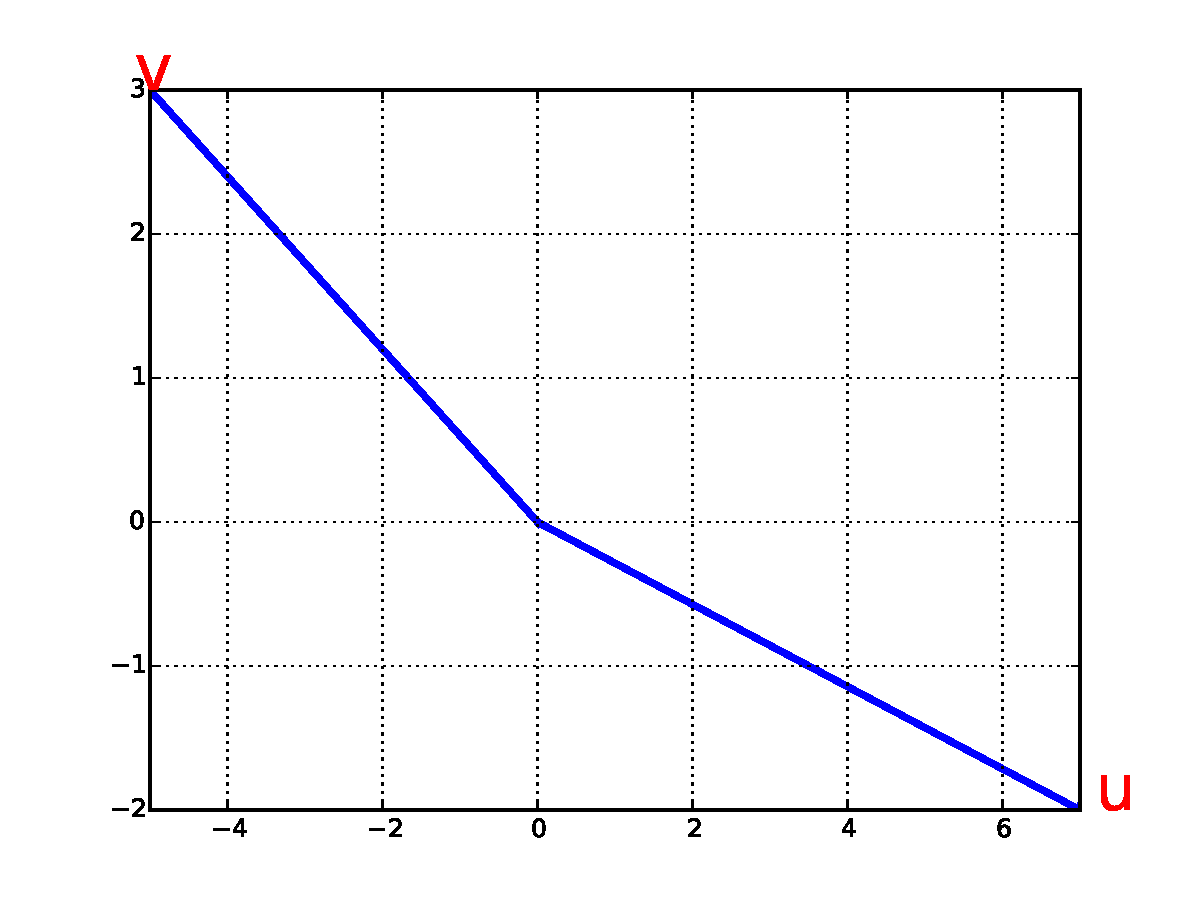
\includegraphics[width=\linewidth]{figs/ex2_1_6.pdf}

\begin{verbatim}
u= Matrix(2, 1, [7, -2])
v= Matrix(2, 1, [-5, 3])

plt.text(float(u[0])+0.2, float(u[1]), 'u', fontsize= 30, color= 'r')
plt.text(float(v[0])-0.2, float(v[1]), 'v', fontsize= 30, color= 'r')
plt.arrow(0, 0, float(u[0]), float(u[1]), lw= 3, color= 'b', head_width=0.05)
plt.arrow(0, 0, float(v[0]), float(v[1]), lw= 3, color= 'b', head_width=0.05)
plt.xlim((-5, 7))
plt.ylim((-2, 3))
plt.grid()
plt.savefig('figs/ex2_1_6.pdf')
plt.close()

(u + v).norm() # sqrt(5)
(u - v).norm() # 13
\end{verbatim}


\subsection{Further Properties of Vectors}
% ========================================

\subsubsection{Exercise 2.2.1}

Find the angle between vectors. The angle is

\begin{equation}\label{eq:uv_angle}
\theta = \arccos(\frac{\mathbf{u} \cdot \mathbf{v}}
{\|\mathbf{u}\| \cdot \|\mathbf{v}\|})
\end{equation}

In \sympy

\begin{verbatim}
def uv_angle(u, v):
    theta= acos(u.dot(v) / (u.norm() * v.norm()))
    return theta
\end{verbatim}

\begin{verbatim}
u= Matrix([1, 1])
v= Matrix([0, 1])
uv_angle(u, v) # pi/4

# As degree:
uv_angle(u, v) * 180/pi # 45

u= Matrix([-1, 2, 3])
v= Matrix([sqrt(2), 1/sqrt(2), -1])
uv_angle(u, v) * 180/pi # ~115 deg
\end{verbatim}

\subsubsection{Exercise 2.2.4}
% ----------------------------
Determine the vector of $k$ so that the vectors are orthogonal to each other.

We want to set the angle between vector equal to 0, \emph{i.e.} Eq. \ref{eq:uv_angle} = 0.

\begin{verbatim}
k= symbols('k', real= True)
u= Matrix([-1, 5, k])
v= Matrix([-3, 2, 7])

eq= Eq(u.dot(v) / (u.norm() * v.norm()) , cos(pi/2))
sol= solve(eq)

# Check
u.subs(k, sol[0]).dot(v) == 0 # True
\end{verbatim}

\subsubsection{Exercise 2.2.6}
% ----------------------------

A vector is normalized by dividing it by its norm. A normalized vector is called
\textbf{unit vector}. In \sympy normlaize with:

\begin{verbatim}
def norm_u(u):
    return u / u.norm()
\end{verbatim}

Determine the value of $k$ so that $\mathbf{\hat{u}} = (1/\sqrt{2}\ 1/2\ k)^T$.

For \textbf{u} to be unit vector, its norm must equal 1. So $\mathbf{\|u\|} = \sqrt{\left\lvert{k}\right\rvert^{2} + 0.75} = 1$.
Solved for $k= \pm 1/2$.

\begin{verbatim}
u= Matrix([1/sqrt(2), 1/2, k])
eq= Eq(u.norm(), 1)
ksol= solve(eq) # [-0.5, 0.5]
\end{verbatim}

\subsubsection{Exercise 2.2.12: Support vector machine}
% -----------------------------------------------------

Find the shortest distance between the vector \textbf{u} and the corresponding
hyperplane. The hyperplane is defined as $\mathbf{v \cdot x} + c = 0$ where
\textbf{v} is a vector of coefficents for the variables in vector \textbf{x} and
$c$ is a constant term. The vector \textbf{u} might represent a data point in
$n$-dimensions.

Remember that an equation in the usual form
$$ax + by +cz + k = 0$$
can be represented in matrix form as
$$ax + by +cz + k
= \left[\begin{matrix}a\\b\\c\end{matrix}\right] \cdot \left[\begin{matrix}x\\y\\z\end{matrix}\right] + k
= \mathbf{v} \cdot \mathbf{x} + k
= 0$$

The shortest distance between \textbf{u} and hyerplane is given by

\begin{equation}\label{eq:ex2_2_12_svm}
d_{shortest} = \frac{|\mathbf{u \cdot v} + c|}{\|\mathbf{v}\|}
\end{equation}

Given \textcolor{red}{$\mathbf{u} = (1\ 1)^T$} and hyperplane \textcolor{blue}{$y= x + 1$}, find the shortes
distance. For this we need to extract the vector of coefficents \textbf{v} from $y= x + 1$, which for convenience can be
re-arranged as $x - y + 1 = 0$.
The coeffients \textbf{v} are $\left[\begin{matrix}1\ \mathit{x} \\ -1\ \mathit{y} \end{matrix}\right]$.

Putting it all together:

\begin{equation}
d_{shortest} = \frac{
    |\left[\begin{matrix}1\\1\end{matrix}\right] \cdot \left[\begin{matrix}1\\-1\end{matrix}\right] + 1|
}{
    \|\left[\begin{matrix}1\\-1\end{matrix}\right]\|
} = \frac{\sqrt{2}}{2} \approx 0.707
\end{equation}

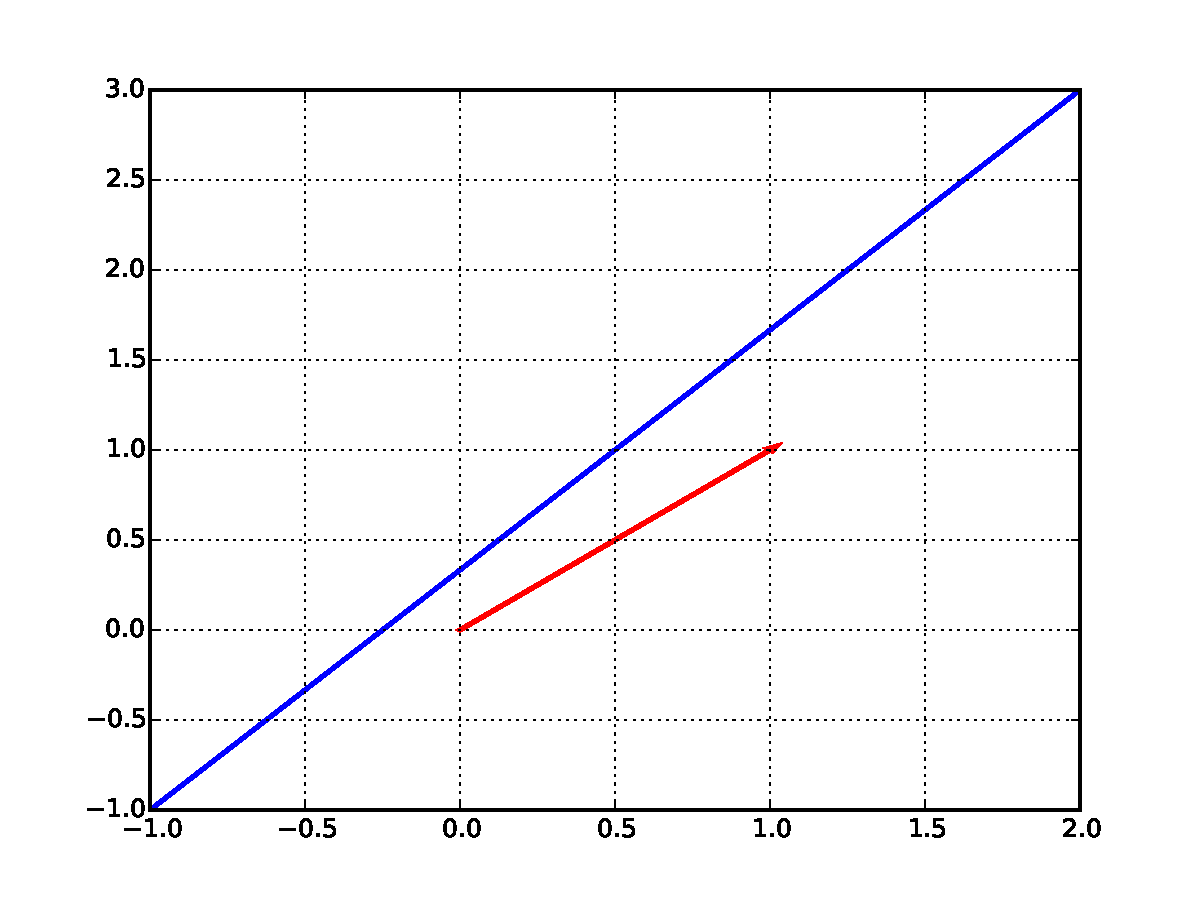
\includegraphics[width=0.75\linewidth]{figs/ex2_2_12_svm.pdf}

\begin{verbatim}
u= Matrix([1, 1])
hyp= Eq(x + 1, y)

# 1. Re-arrange hyp to have x + y + c= 0
hyp2= Eq(hyp.lhs - hyp.rhs)

# 2. Re-arrange in matrix form
cfdict= hyp2.lhs.as_expr().as_coefficients_dict()
v= Matrix([cfdict[x], cfdict[y]])
c= cfdict[numbers.One()]
d_shortest= abs(u.dot(v) + c) / v.norm()
\end{verbatim}

Plotted with:

\begin{verbatim}
plt.plot([-1, 2], [hyp.lhs.subs(x, -2), hyp.lhs.subs(x, 2)], 'b-', lw= 2)
plt.arrow(0, 0, float(u[0]), float(u[1]), lw= 2, color= 'red')
plt.grid()
plt.xlim([-0.5, 1.5])
plt.ylim([-0.5, 1.5])
plt.savefig('figs/ex2_2_12_svm.pdf')
plt.close()
\end{verbatim}

\subsubsection{Exercise 2.2.12d}
% ------------------------------

For $\mathbf{u} = \left[\begin{matrix}1\\2\\3\\4\end{matrix}\right]$ and
$x + 2y + z + w = 10$. We have

$$
d_{shortest}
= \frac{|\mathbf{u} \cdot \mathbf{v} + c|}{\|\mathbf{v}\|}
= \frac{|\left[\begin{matrix}1\\2\\3\\4\end{matrix}\right] \cdot \left[\begin{matrix}1\\2\\1\\1\end{matrix}\right] - 10|}{\|\left[\begin{matrix}1\\2\\1\\1\end{matrix}\right]\|}
= \frac{2 \sqrt{7}}{7}
\approx 0.76
$$

\begin{verbatim}
x,y,z,w = symbols('x y z w')
u = Matrix([1,2,3,4])
hyp= Eq(x + 2*y + z + w, 10)

hyp= hyp.lhs - hyp.rhs
v= [hyp.as_coefficients_dict()[t] for t in (x, y, z, w)]
v= Matrix(v)
c= hyp.as_coefficients_dict()[numbers.One()]

d_shortest= abs(u.dot(v) + c) / v.norm()
\end{verbatim}

\subsection{Linear Independence}
% ==============================

\subsubsection{Exercise 2.3.1}
% ----------------------------

Determine which vectors in $\mathbb{R}^2$ are \textbf{linearly dependent}.

The linear combination of vectors \textbf{u} and \textbf{v} is

\begin{equation}\label{eq:ex2_3_1}
k\mathbf{u} + c\mathbf{v} = \mathbf{O}
\end{equation}

Or more verbose:

\begin{equation}\label{eq:ex2_3_1_II}
k \left[\begin{matrix}x_1\\x_2\end{matrix}\right] +
c \left[\begin{matrix}y_1\\y_2\end{matrix}\right] =
\left[\begin{matrix}0\\0\end{matrix}\right]
\end{equation}

Where $k$ and $c$ are scalars (unknown coefficients). If \ref{eq:ex2_3_1} is
satisfied for $k \neq 0$ or $c \neq 0$ then \textbf{u} and \textbf{v} are
linearly dependent. Which means that \textbf{u} can be expressed as \textbf{v} times
a scalar, or vice versa.

Expressed as a system of equations, \ref{eq:ex2_3_1_II} becomes:

\begin{equation}
\begin{matrix}
kx_1 + cy_1 = 0 \\
kx_2 + cy_2 = 0
\end{matrix}
\end{equation}

Now solve this system and check whether $k=0$ and $c=0$ are the only solutions.

For $\mathbf{u} = \left[\begin{matrix}6\\10\end{matrix}\right]$  and
$\mathbf{v} = \left[\begin{matrix}-3\\-5\end{matrix}\right]$ we have:

$$
k \left[\begin{matrix}6\\10\end{matrix}\right] + c \left[\begin{matrix}-3\\-5\end{matrix}\right] = \left[\begin{matrix}0\\0\end{matrix}\right]
$$

re-arranged as a system

$$
\begin{matrix}6 k - 3 c = 0\\10 k - 5 c = 0\end{matrix}
$$

With solutions $\begin{bmatrix}\begin{Bmatrix}k : \frac{c}{2}\end{Bmatrix}, & \begin{Bmatrix}c : 2 k\end{Bmatrix}\end{bmatrix}$
which hold for $c$ and $k$ different from 0.

\begin{verbatim}
u= Matrix([6, 10])
v= Matrix([-3, -5])
eq1= Eq(k * u[0] + c * v[0], 0)
eq2= Eq(k * u[1] + c * v[1], 0)

csol= solve([eq1, eq2], c)
ksol= solve([eq1, eq2], k)
\end{verbatim}

Note that the conclusion of linear dependence can be reached by looking at the
rank of the matrix $\mathbf{A}= \left[\begin{matrix}\mathbf{u} & \mathbf{v}\end{matrix}\right]$.
In fact, $rank(\mathbf{A})$ is less than 2.

$$
\mathbf{A} = \left[\begin{matrix}\mathbf{u} & \mathbf{v}\end{matrix}\right]
= \left[\begin{matrix}6 & -3\\10 & -5\end{matrix}\right]
$$

with $rank(\mathbf{A}) = 1$. Note that trying to solve \textbf{A} results in
\sympy error \textcolor{red}{\texttt{ValueError: Matrix det == 0; not invertible.}}

In addition, note that the RREF has only one leading row:

$$
\mathbf{A_{rref}} = \begin{pmatrix}\left[\begin{matrix}1 & - \frac{1}{2} & 0\\0 & 0 & 0\end{matrix}\right], & \begin{bmatrix}0\end{bmatrix}\end{pmatrix}
$$

\begin{verbatim}
A= v.col_insert(0, u)
A_rank= A.rank() # 1

try:
    A.solve(Matrix([0, 0])) # Matrix det == 0; not invertible.
except ValueError, e:
    print e
    
A_rref= A.col_insert(2, Matrix([0,0])).rref()
\end{verbatim}

Unit vectors $\mathbf{e_1} = \left[\begin{matrix}1\\0\end{matrix}\right]$ and
$\mathbf{e_2} = \left[\begin{matrix}0\\1\end{matrix}\right]$ are linearly independent.
Note that $rank(\mathbf{A}) = N_{dimensions} = 2$ and the RREF is complete

$$
\mathbf{A_{rref}} = \begin{pmatrix}\left[\begin{matrix}1 & 0 & 0\\0 & 1 & 0\end{matrix}\right], & \begin{bmatrix}0, & 1\end{bmatrix}\end{pmatrix}
$$

\begin{verbatim}
k, c= symbols('k c')
e1= Matrix([1, 0])
e2= Matrix([0, 1])

eq1= Eq(k * e1[0] + c * e1[1], 0)
eq2= Eq(k * e2[0] + c * e2[1], 0)

solve([eq1, eq2]) # {c: 0, k: 0}

# Also
A= e2.col_insert(0, e1)
A_rank= A.rank() # 2

A_rref= A.col_insert(2, Matrix([0,0])).rref()
\end{verbatim}

\subsubsection{Exercise 2.3.12 - \textit{incomplete}}
% ---------------------------------------------------

Determine the value of $t$ in the \textbf{linearly independent} vectors

$$
\mathbf{u} = \left[\begin{matrix}t\\1\\1\end{matrix}\right],
\mathbf{v} = \left[\begin{matrix}-1\\t\\1\end{matrix}\right],
\mathbf{w} = \left[\begin{matrix}1\\1\\t\end{matrix}\right],
$$

The RREF of the augmented matrix is:

$$
\mathbf{A_{rref} = \begin{pmatrix}\left[\begin{matrix}1 & 0 & 0 & 0\\0 & 1 & 0 & 0\\0 & 0 & 1 & 0\end{matrix}\right], & \begin{bmatrix}0, & 1, & 2\end{bmatrix}\end{pmatrix}}
$$

which implies that either the coefficients $k_1 = k_2 = k_3 = 0$ or $t$

\begin{verbatim}
t, k1, k2, k3= symbols('t k1 k2 k3', real= True)

u= Matrix([ t, 1, 1]) # k1
v= Matrix([-1, t, 1]) # k2
w= Matrix([ 1, 1, t]) # k3

eq1= Eq(k1*t - k2   + k3,   0)
eq2= Eq(k1   + k2*t + k3,   0)
eq3= Eq(k1   + k2   + k3*t, 0)

A= w.col_insert(0, v).col_insert(0, u)
Au= Matrix([0,0,0]).col_insert(0, A)
A_rref= Au.rref()
\end{verbatim}

\subsection{Basis and Spanning Set}
% =================================

\subsubsection{Example 2.17}
% ----------------------------

Determine whether the vectors $\mathbf{u} = \left[\begin{matrix}1\\2\end{matrix}\right]$
and $\mathbf{v} = \left[\begin{matrix}-1\\1\end{matrix}\right]$ \textbf{span} $\mathbb{R}^2$.
In other words, the question is whether with the axis \textbf{u} and \textbf{v}
we can draw any vector in $\mathbb{R}^2$. In other words again, can any vector in
$\mathbb{R}^2$ be defined as a \emph{\textbf{linear combination}} of \textbf{u} and \textbf{v}?

So let's take a generic vector in $\mathbb{R}^2$ $\mathbf{w} = \left[\begin{matrix}a\\b\end{matrix}\right]$
and see if the equation

\begin{equation}\label{eq:example_2_17}
\mathbf{w} = k\mathbf{u}  + c\mathbf{v}
\end{equation}

can be solved to find the coefficients \textbf{k} and \textbf{c}.
If the answer is yes, than the generc vector \textbf{w} can be defined in terms
of \textbf{u} and \textbf{v} given appropriate coefficients $k$ and $c$ respectively.

To solve \ref{eq:example_2_17} build the augmented matrix

$$\mathbf{A} =
\left[\begin{matrix}1 & -1 & a\\2 & 1 & b\end{matrix}\right]$$,

put in RREF and see if the RREF is complete. In this case

$$\mathbf{A_{rref}} = \left[\begin{matrix}1 & 0 & \frac{a}{3} + \frac{b}{3}\\0 & 1 & - \frac{2 a}{3} + \frac{b}{3}\end{matrix}\right]$$

The coefficients \textbf{k} and \textbf{c} are given as the last column

\begin{equation}\label{eq:example_2_17_ii}
k, c= \left[\begin{matrix}\frac{a}{3} + \frac{b}{3}\\- \frac{2 a}{3} + \frac{b}{3}\end{matrix}\right]
\end{equation}

Here $a$ and $b$ can be thought as increments on the $x$ and $y$ axis.

For example, how do we express the vector $\mathbf{g} = \left[\begin{matrix}3\\2\end{matrix}\right]$
in the \textbf{spanning set} \textbf{u} and \textbf{v}? By substituting in \ref{eq:example_2_17_ii}
3 for $a$ and 2 for $b$ we get the coefficients $k= 5/3$ and $c = -4/3$. Therefore

\begin{align}
\mathbf{g} = \left[\begin{matrix}3\\2\end{matrix}\right]
= k\mathbf{u} + c\mathbf{v} \\
= \left[\begin{matrix}\frac{a}{3} + \frac{b}{3}\end{matrix}\right] \mathbf{u} + \left[\begin{matrix}- \frac{2 a}{3} + \frac{b}{3} \mathbf{v}\end{matrix}\right] \\
= \left[\begin{matrix}\frac{3}{3} + \frac{2}{3}\end{matrix}\right] \mathbf{u} + \left[\begin{matrix}- \frac{2 \cdot 3}{3} + \frac{2}{3} \mathbf{v}\end{matrix}\right] \\
= 5/3 \mathbf{u} + -4/3 \mathbf{v} \\
= \left[\begin{matrix}3\\2\end{matrix}\right]
\end{align}

\begin{verbatim}
a,b,c,k= symbols('a b c k')

u= Matrix([1, 2])
v= Matrix([-1, 1])
w= Matrix([a, b])

A= w.col_insert(0, v).col_insert(0, u)
A_rref= A.rref()

# Coefficients
k, c= A_rref[0].col(- 1)

# Or maybe easier using M.solve(const)
A= v.col_insert(0, u)
k, c= A.solve(w)

## Represent g in spanning set (u, v)
g= Matrix([3, 2])
k2= k.subs({a:g[0], b:g[1]})
c2= c.subs({a:g[0], b:g[1]})
g2= k2 * u + c2 * v
\end{verbatim}

\subsubsection{Exercise 2.4.1}
% ----------------------------

Determine whether the following vectors span $\mathbb{R}^2$

\begin{verbatim}
# Generic vector
w= Matrix([a, b])

e1= Matrix([1, 0])
e2= Matrix([0, 1])

A= w.col_insert(0, e2).col_insert(0, e1)
\end{verbatim}

For unit vectors $\mathbf{e_1}$ and $\mathbf{e_2}$ the answer is yes with
coefficient a and b from RREF

$$
\mathbf{A_{rref}} = \left[\begin{matrix}1 & 0 & a\\0 & 1 & b\end{matrix}\right]
$$

These vectors do not form a spanning set as a generic vector \textbf{w} cannot be formed
by linear combination. The augmented matrix cannot be in RREF:

$$
\mathbf{A_{rref}} = \left[\begin{matrix}1 & - \frac{1}{2} & 0\\0 & 0 & 1\end{matrix}\right]
$$

Trying to solve the augmented matrix \textcolor{red}{\texttt{ValueError: Matrix det == 0; not invertible.}}

$$
\mathbf{A} = \left[\begin{matrix}2 & -1 & a\\2 & -1 & b\end{matrix}\right]
$$

Results in 

\begin{verbatim}
u= Matrix([2, 2])
v= Matrix([-1, -1])
A= w.col_insert(0, v).col_insert(0, u)
A.rref() # Not in RREF

# Indeed:
A= v.col_insert(0, u)
A.solve(w) # ValueError: Matrix det == 0; not invertible.
\end{verbatim}

\subsubsection{Exercise 2.4.2}
% ----------------------------

Determine whether the following vectors span $\mathbb{R}^3$

\begin{verbatim}
u= Matrix([1, 2, 1])
v= Matrix([2, 4, 0])
w= Matrix([-2, -2, 3])
\end{verbatim}

So, let's define a generic vector in $\mathbb{R}^3$

\begin{verbatim}
a,b,c= symbols('a b c')
g= Matrix([a, b, c])
\end{verbatim}

and define \textbf{g} as a linear combination of \textbf{u, v, w}
\emph{i.e.}
$$ \mathbf{g}= k\mathbf{u} + j\textbf{v} + l\mathbf{w}$$

Can we solve these linear system to find the unknow $k, j, l$?

To answer, prepare the augmented matrix (not really necessary to prepare it though).
Note the use of \texttt{numpy.hstack} to column-bind vectors. Now try to solve it

\begin{verbatim}
A= Matrix(numpy.hstack((u, v, w, g)))
sol= A[:, :-1].solve(A[:, -1])
\end{verbatim}

The syntax to slice the matrix comes from \href{http://docs.scipy.org/doc/numpy/reference/arrays.indexing.html}{NumPy}:
\textcolor{blue}{\texttt{A[:, :-1]}} means get all rows with ':' (1st index) and all columns
excluding the last one with ':-1'.

Anyway, the solution exists and is

$$
k, j, l= \left[\begin{matrix}3 a - \frac{3 b}{2} + c\\- 2 a + \frac{5 b}{4} - \frac{c}{2}\\- a + \frac{b}{2}\end{matrix}\right]
$$

so \textbf{u, v, w} are spanning set of $\mathbb{R}^3$

\subsubsection{Exercise 2.4.3}
% ----------------------------

Determine whether the following vectors form a \textbf{\textit{basis}} for $\mathbb{R}^2$

\begin{verbatim}
u= Matrix([1, 2])
v= Matrix([0, 1])
\end{verbatim}

A \textbf{\textit{basis}} is a spanning set whose vectors are also linearly independent.
This means that a basis is the minimal set of vectors necessary to describe the
$\mathbb{R}^n$ space. Note that if the vectors span $\mathbb{R}^n$ than they are
linearly independent and \emph{vice versa}. So we need to check only one of the two
conditions.

In the case above we have linearl independence since:

$$
A = \left[\begin{matrix}u\\v\end{matrix}\right]
= \left[\begin{matrix}0 & 1\\1 & 2\end{matrix}\right]
$$

and a solution can be found:

$$
a, b= \left[\begin{matrix}- 2 a + b\\a\end{matrix}\right]
$$

\begin{verbatim}
A= Matrix(numpy.array((u, v)))
sol= A.solve(Matrix([a, b]))
A.rank() == A.rows # True (2)
A.det() != 0 # True
A.rref() 
\end{verbatim}

Note also that $rank(A) = 2$, \emph{i.e.} \textbf{A} is full rank and the RREF
is complete $\left[\begin{matrix}1 & 0\\0 & 1\end{matrix}\right]$

In this case, there is no linear independence and the vectors are not a basis:

\begin{verbatim}
u= Matrix([-2, -4])
v= Matrix([1, 2])
A= Matrix(numpy.array((u, v)))
sol= A.solve(Matrix([a, b]))  ## ValueError: Matrix det == 0; not invertible.
A.rank() == A.rows # False
A.det() == 0 # True
\end{verbatim}

\subsubsection{Exercise 2.4.4}
% ----------------------------

Do these vector form a basis for $\mathbb{R}^4$?

\begin{verbatim}
u= Matrix([1, 1, 1, 1])
v= Matrix([1, 1, 0, -1])
w= Matrix([-1, -2, -3, 4])
x= Matrix([2, 2, 2, 2])
A= Matrix(numpy.hstack([u, v, w, x]))
\end{verbatim}

No since they are not linearly independent. In fact u and x are multiple of each other.

\subsubsection{Exercise 2.4.5}
% ----------------------------

Is \textbf{b} in the space spanned by the columns of matrix \textbf{A}?

\begin{equation}
\mathbf{A} = \left[\begin{matrix}1 & 1 & 0\\2 & 5 & 0\\3 & 4 & 9\end{matrix}\right];
\mathbf{b} = \left[\begin{matrix}1\\3\\4\end{matrix}\right]
\end{equation}

To answer we want to know whether the columns of \textbf{A} can be linearly combined
to produce \textbf{b}. Can we found a vector \textbf{k} of coefficients for the
columns in \textbf{A} that produce \textbf{b}?
So we want ot see if we can solve $\mathbf{Ak} = \mathbf{b}$ \emph{w.r.t.} \textbf{k}.
\emph{I.e.} let's try to solve $\mathbf{k}= \mathbf{A}^{-1}\mathbf{b}$. We can solve it
for $\mathbf{k} = \left[\begin{matrix}\frac{2}{3}\\\frac{1}{3}\\\frac{2}{27}\end{matrix}\right]$.

We can also verify that $\mathbf{Ak} = \mathbf{b}$.

\begin{verbatim}
A= Matrix([[1, 1, 0], [2, 5, 0], [3, 4, 9]])
b= Matrix([1, 3, 4])

k= A.inv().dot(b)
# The same:
k= A.solve(b)

# Check back:
b == Matrix(A.dot(k))
\end{verbatim}

What about this case:

\begin{verbatim}
A= Matrix([[1, 2, 3],
           [4, 5, 6],
           [7, 8, 9]])
b= Matrix([1, 3, 4])
A.inv() ## ValueError: Matrix det == 0; not invertible.
A.solve(b) ## The same
\end{verbatim}

\texttt{ValueError: Matrix det == 0; not invertible}, in fact the columns of \textbf{A}
are not linearly independent we cannot find a vector of coefficients \textbf{k} 
to represent \textbf{b}.

\begin{verbatim}
\end{verbatim}

\subsubsection{Exercise 2.4.6}
% ----------------------------

Are these vectors a basis for $mathbb{R}^3$?

\begin{verbatim}
u= Matrix([5, 0, 0])
v= Matrix([0, 6, 0])
w= Matrix([0, 0, 7])
A= Matrix(numpy.hstack([u, v, w]))
A.solve(Matrix([a, b, c])) ## Solvable -> lin. indep. -> basis
\end{verbatim}

What about:

\begin{verbatim}
alpha, beta, lamda= symbols('alpha beta lamda', real= True, nonzero= True)
u= Matrix([alpha, 0, 0])
v= Matrix([0, beta, 0])
w= Matrix([0, 0, lamda])
A= Matrix(numpy.hstack([u, v, w]))
A.solve(Matrix([a, b, c])) ## Solvable -> lin. indep. -> basis

# Also:
A.inv() # Ok
A.rank() == 3 # True
A.det() != 0 # True
\end{verbatim}

\subsubsection{Exercise 2.4.9}
% ----------------------------
